% !TeX root = ../solution.tex

\hypertarget{he22.29}{%
\chapter{[HE22.29] Layer Cake}\label{he22.29}}

\begin{marginfigure}
	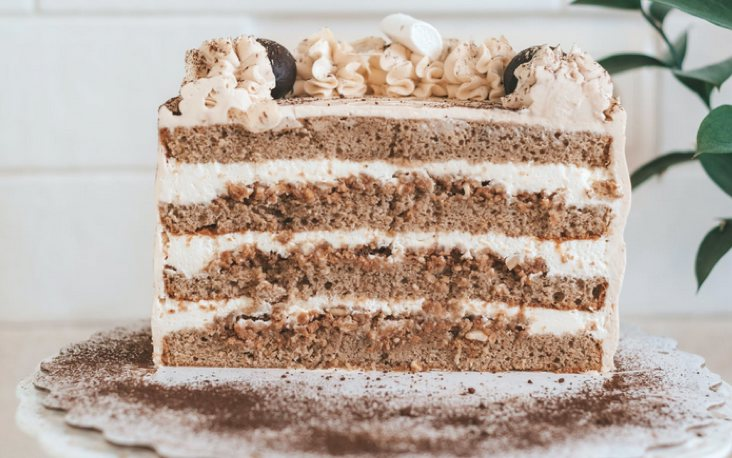
\includegraphics[width=49mm]{level7/challenge29.jpg}
\end{marginfigure}
\section{Intro}
Someone said there would be cake.\\
\noindent\verb+{hackyeaster/layercake:latest}+


\section{Hint}
Docker Hub

\section{Solution}\label{hv22.29solution}

As per the hint, the input is a docker image.  Looking at it in Docker Desktop,
we see that it has many layers and in each a file
\texttt{app/egg.png} should be present.  Probably one of them is the flag.

Save the docker image to a tar file with 
\texttt{docker save -o container.tar hackyeaster/layercake} and extract it.  This
generates many directories, but each contains a file \verb+layer.tar+ that
contains all the data for this layer.  So all we have to do is to extract all
the \verb+layer.tar+ and look all \verb+egg.png+ files.  A little script helps

\begin{marginfigure}
	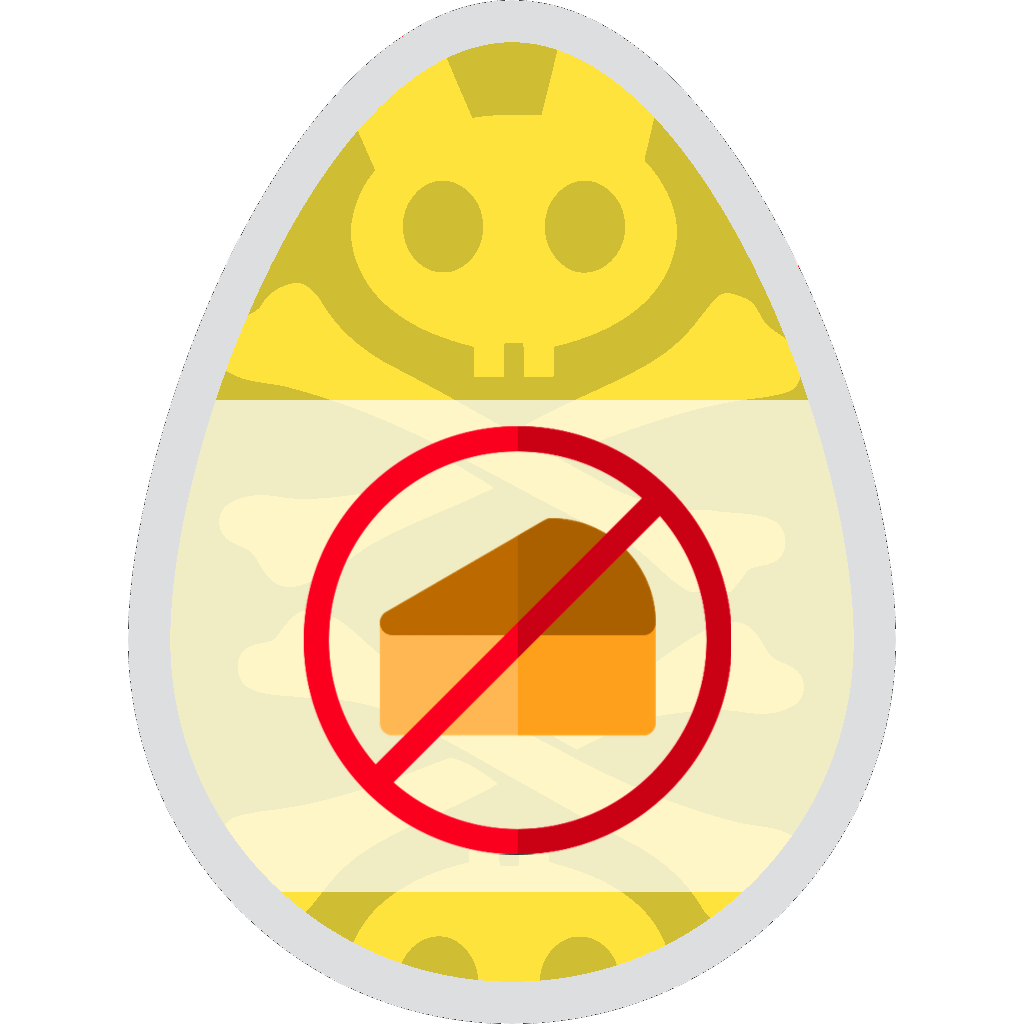
\includegraphics[width=49mm]{level7/egg_0.png}
\end{marginfigure}

\begin{minted}{python}
import tarfile
import glob
import os
import os.path

index = 0
for f in glob.glob('*/layer.tar'):
    tf = tarfile.open(f)
    tf.extractall('.')
    tf.close()
    if os.path.exists('app/egg.png'):
        os.rename('app/egg.png', f'app/egg_{index}.png')
    index += 1
\end{minted}

Amongst the files are many that are broken eggs, but one contains the flag \verb+he2022{th3_c4k3_is_a_l1e!}+.

\begin{marginfigure}
	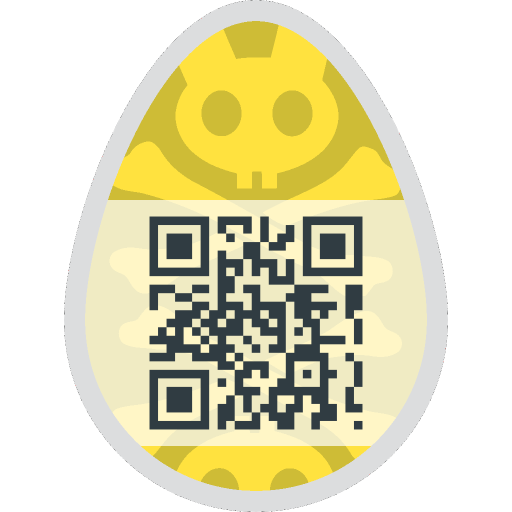
\includegraphics[width=49mm]{level7/egg_12.png}
\end{marginfigure}




	









